\chapter{Progettazione}
\label{cap:progettazione}

\intro{In questo capitolo verrà illustrata la fase di progettazione del prodotto, partendo dalla realizzazione di un mockup, passando per la definizione dell'architettura e le tecnologie da utilizzare.}\\

\section{Mockup}
\label{sec:mockup}

Il primo passo per la progettazione dell'applicazione è stato quello di realizzare un \gls{mockup}\glsoccur con lo scopo di definirne il più dettagliatamente possibile l'interfaccia grafica: il numero di viste necessarie, la loro struttura, i componenti grafici e la loro disposizione, la \emph{palette} dei colori, come l'utente interagirà con l'applicazione e come questa dovrà rispondere a tali interazioni simulabili attraverso un prototipo. Infatti, per l'implementazione della \gls{uig}\glsoccur si è rivelato essere di notevole utilità, in quanto ha reso più semplice e veloce la realizzazione di quest'ultima, avendo compreso a priori come questa dovesse essere strutturata.\\
Inoltre il \gls{mockup} è stato utilizzato per definire le funzionalità che l'applicazione deve offrire, in modo da avere un'idea più chiara di come queste debbano essere implementate e, infine, come è stato menzionato nella sezione \ref{subsec:variazione-pianificazione}, è stato indispensabile per la fase di \emph{analisi dei requisiti} .\\ 
Si specifica che nel corso della fase di implementazione sono state apportate delle modifiche all'interfaccia grafica per migliorarne l'usabilità, mantenendo però invariata la struttura generale dell'applicazione e prestando particolare attenzione all'esperienza utente, in modo da rendere l'utilizzo dell'applicazione, in mobilità, il più semplice e intuitivo possibile.\\
|| FORSE, HA SENSO METTERE IN CONFRONTO IL MOCKUP E REALE UI ? ||\\
Di seguito dunque vengono presentate le schermate che compongono il mockup dell'applicazione, con una breve descrizione riguardanti le funzionalità che esse offrono e i componenti grafici che la compongono, con lo scopo di rendere più chiara la loro funzione e il loro utilizzo. 

\subsection{Schermata di login}
\label{subsec:login}


\section{Architettura}
\label{sec:architettura}
% State Management -> RIVERPOD + Diagramma illustrativo
% https://codewithandrea.com/articles/flutter-app-architecture-riverpod-introduction/

\subsection{Architettura Flutter}
\label{subsec:architettura-flutter}

Per comprendere al meglio la peculiarità di \emph{Flutter} descritta nella sezione \ref{subsec:flutter} è necessario analizzare l'architettura\cite{site:flutter-architecture} delle applicazioni realizzate con essa, che sono composte dagli elementi illustrati nella figura \ref{fig:architettura-flutter}, tra i quali, i principali sono descritti di seguito:
\begin{itemize}
    \item \textbf{Embedder}: fornisce un punto d'ingresso con il sistema operativo ospitante per accedere ai servizi forniti da esso. Questo consente dunque l'esecuzione dell'applicazione su diverse piattaforme e la possibilità di utilizzare librerie per accedere a funzionalità esclusive di determinati sistemi operativi, oppure viceversa, integrare il codice \emph{Flutter} in un'applicazione nativa già esistente;
    \item \textbf{Flutter engine}: è il componente centrale che fornisce l'implementazione di basso livello dell'\gls{apig}\glsoccur principale di \emph{Flutter}, inclusa la grafica, il layout di testo, operazioni di \emph{I/O}, rete, ecc.;
    \item \textbf{Flutter framework}: componente con il quale lo sviluppatore interagisce attraverso un insieme di librerie, che partendo dal basso sono:
    \begin{itemize}
        \item \textbf{foundation}: fornisce un'astrazione delle funzionalità di animazione, grafica e \gls{gesture}\glsoccur;
        \item \textbf{rendering}: fornisce un'astrazione per gestire il layout. Con questo livello è possibile costruire un albero di oggetti renderizzabili.
        \item \textbf{widget}: ogni oggetto renderizzabile ha una classe corrispondente in questa libreria, definiti appunto \emph{widget}, l'unità fondamentale in \emph{Flutter}, che permettono la realizzazione dell'interfaccia grafica;
        \item \textbf{Material e Cupertino}: forniscono un'implementazione di alto livello dei \emph{widget} per la realizzazione di interfacce grafiche seguendo le linee guida di \emph{Material Design} e \emph{Cupertino}, rispettivamente per le piattaforme \emph{Android} e \emph{iOS}.
    \end{itemize}
    \item \textbf{Dart App}: codice sorgente sviluppato dall'utente, contenente i \emph{widget} per l'implementazione della \gls{uig}\glsoccur e la logica dell'applicazione.
\end{itemize}

Inoltre, essendo un \gls{framework}\glsoccur \gls{open-source}\glsoccur, è possibile utilizzare librerie di terze parti, sviluppate dalla community, per aggiungere funzionalità all'applicazione, come ad esempio librerie per la gestione dello stato dell'applicazione, librerie per la gestione delle richieste HTTP, ecc. \\

\begin{figure}[!h] 
    \centering 
    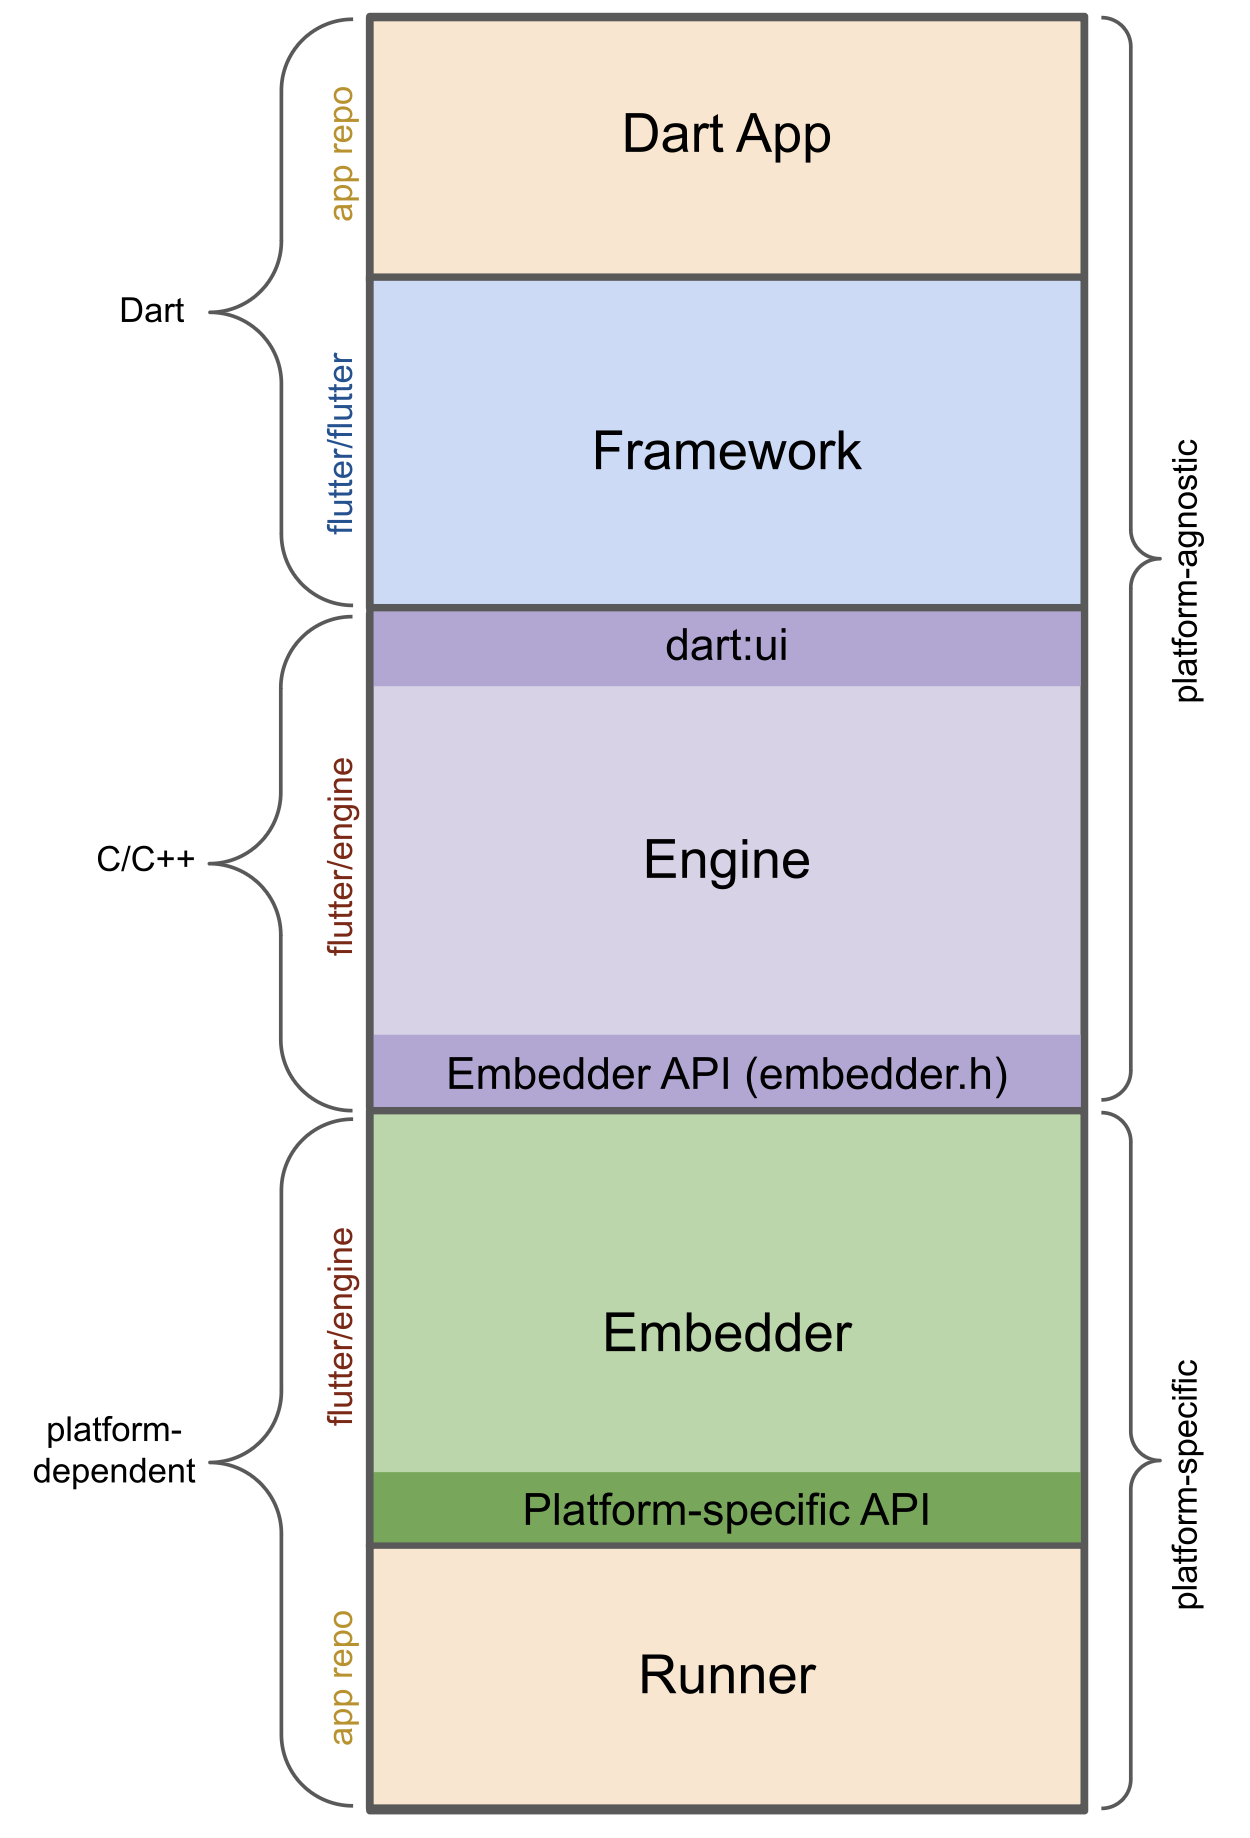
\includegraphics[width=0.4\columnwidth]{images/flutter-app-anatomy.png} 
    \caption{Struttura di un'applicazione in \emph{Flutter}.}
    \label{fig:architettura-flutter}
\end{figure}

Lo stato posseduto dai \lstinline{StatefulWidget} (vedi sezione \ref{subsec:flutter}) può essere considerato come \emph{ephemeral} (ing. effimero) o \emph{app state} (ing. stato dell'applicazione). \\
\emph{Ephemeral} è uno stato che può essere opportunamente confinato all'interno di un singolo \emph{widget} e gestito attraverso la primitiva \lstinline{setState()}, che permette di definire come aggiornarlo.\\
Mentre \emph{app state} è uno stato che viene condiviso tra più \emph{widget} e per la sua gestione, più complessa utilizzando solamente la primitiva sopra citata, esistono diverse librerie di terze parti, ciascuna con le proprie peculiarità a seconda del caso d'uso.\\
\indent La problematica di come gestire lo stato dell'applicazione è definito in gergo \emph{state management}\cite{site:flutter-state-mgmt}, e dopo un'attenta analisi delle librerie disponibili, si è scelto di utilizzare \emph{Riverpod}\cite{site:riverpod}.\\

\subsection{Riverpod}
\label{subsec:riverpod}

\emph{Riverpod} semplifica notevolmente lo \emph{state management} e si basa su un concetto evoluto da \emph{Provider}\cite{site:provider}, libreria da cui deriva.\\
A differenza di \lstinline{InheritedWidget}\cite{site:inheritw} che permette di condividere lo stato tra più \emph{widget}, \emph{Riverpod}, che ne è una reimplementazione, fornisce \emph{providers} che sono indipendenti dai \emph{widget}, in quanto una volta dichiarato il \lstinline{ProviderScope} a livello globale, possono essere letti ovunque, a condizione che la classe richiamante venga estesa con \lstinline{ConsumerWidget} o \lstinline{ConsumerStatefulWidget}\cite{site:reading-provider}. \\
Da questo ne consegue che si evita di aggiornare l'interfaccia grafica, ovvero di richiamare il metodo \lstinline{build()} di un \emph{widget} quando non è necessario, poichè è un'operazione costosa.
Un \emph{provider} dunque è un oggetto che può essere richiamato da un \emph{widget} con la finalità di leggerne un valore.\\
Ne esistono di varie tipologie, per le quali si rimanda alla documentazione ufficiale\cite{site:riverpod}, ma quelle utilizzate in questo progetto sono:
\begin{itemize}
    \item \lstinline{FutureProvider}: utilizzato per ricevere un valore generato da un'operazione asincrona (es: richiesta \gls{httpg}\glsoccur);
    \item \lstinline{StateNotifierProvider}: utilizzato per gestire una classe che mantiene uno stato, più complesso di una semplice variabile primitiva, e di esporre dei metodi per monitorarlo o aggiornarlo.
\end{itemize}

\subsection{Architettura dell'applicazione}
\label{subsec:architettura-app}

Per l'architettura dell'applicazione si è scelto di utilizzare un \emph{pattern} architetturale basato su \gls{mvcg}\glsoccur, che permette di separare la logica dell'applicazione dalla sua rappresentazione grafica, in modo da rendere più semplice la manutenzione e l'aggiunta di nuove funzionalità.\\
Nel dettaglio l'applicazione è composta da quattro livelli:
\begin{itemize}
    \item \textbf{Data Layer}: contiene le classi che si occupano di recuperare i dati dal server, attraverso richieste \gls{httpg}\glsoccur, e di convertirli in oggetti rappresentati nel \emph{domain layer};
    \item \textbf{Domain Layer}: contiene le classi che rappresentano i dati dell'applicazione;
    \item \textbf{Application Layer}: contiene le classi che si occupano di gestire la logica dell'applicazione;
    \item \textbf{Presentation Layer}: contiene le classi che si occupano di gestire l'interfaccia, ovvero di eseguire il rendering dei \emph{widget} e di gestire gli eventi generati dall'utente.
\end{itemize}
Questa architettura permette inoltre di avere la possibilità di definire eventualmente più sorgenti da cui recuperare i dati senza dover modificare il codice relativo ai livelli superiori, in quanto è sufficiente modificare il \emph{data layer}\cite{site:app-architecture}.\\

\section{Struttura del progetto}
\label{sec:struttura-progetto}
% Struttura del progetto: cartelle, file, ecc. -> LAYER FIRST
Un altro aspettato importante da considerare per la realizzazione di un progetto software è la sua struttura, ovvero come organizzare i file e le cartelle che lo compongono.\\
Dopo opportune ricerche ed analisi, si è scelto di adottare, tra le due alternative disponibili, la struttura \emph{layer first}, che prevede di organizzare i file e le cartelle in base al livello a cui appartengono, in modo da rendere più semplice la manutenzione e l'aggiunta di nuove funzionalità.\\
\emph{Feature first}, l'altra alternativa, organizza invece i file e le cartelle, mantendendo la separazione tra i livelli, in base alle funzionalità che l'applicazione offre.\\
Il motivo principale per cui la scelta non è ricaduta su quest'ultima è che, nonostante sia quella che garantisca un'organizzazione e manutenzione del codice migliore, risulta essere più complessa da implementare in quanto adatta per progetti di dimensione e complessità maggiore.\\
Di seguito verranno illustrati entrambi gli approcci, in modo da poterli confrontare e comprendere meglio le loro differenze\cite{site:project-structure}.\\
\begin{multicols}{2}
    \begin{verbatim}
        // LAYER FIRST
        lib/
            data/
                feature1.dart
                feature2.dart
            domain/
                feature1.dart
                feature2.dart
            application/
                feature1.dart
                feature2.dart
            presentation/
                feature1.dart
                feature2.dart
    \end{verbatim}
    \begin{verbatim}
        // FEATURE FIRST
        lib/
            feature1/
                data.dart
                domain.dart
                application.dart
                presentation.dart
            feature2/
                data.dart
                domain.dart
                application.dart
                presentation.dart
    \end{verbatim}
\end{multicols}

% \section{Diagrammi UML}
% \label{sec:uml}
% dove inserirli?
% UML -> Diagrammi delle classi

% \subsubsection{Namespace 1} %**************************
% Descrizione namespace 1.

% \begin{namespacedesc}
%     \classdesc{Classe 1}{Descrizione classe 1}
%     \classdesc{Classe 2}{Descrizione classe 2}
% \end{namespacedesc}

\section{Ambiente di sviluppo}
\label{sec:ambiente-sviluppo}
% SEGUI ISSUE #4 E #5 PER LA STESURA DI QUESTA SEZIONE
Di seguito viene descritto l'ambiente di sviluppo e data una panoramica delle tecnologie e strumenti utilizzati.

\subsection*{Figma}
\label{subsec:figma}

\emph{Figma}\cite{site:figma} è un software di editor di grafica vettoriale che permette di progettare interfacce grafiche per applicazioni \emph{web} e \emph{mobile}.\\
È stato utilizzato per la realizzazione del \gls{mockup}\glsoccur dell'applicazione, in quanto vi è la possibilità di creare un prototipo interattivo, che simula l'interazione dell'utente con l'applicazione, e di condividerlo con il team di sviluppo, in modo da avere un'idea più chiara di come l'applicazione debba essere strutturata e di come debba funzionare.\\

\subsection*{Git}
\label{subsec:git}

\emph{Git}\cite{site:git} è un sistema di controllo di versione, finalizzato al tracciamento del codice sorgente e delle sue modifiche, inoltre ne permette la condivisione e dunque la collaborazione tra più sviluppatori.\\
Inoltre è possibile, eventualmente, in caso di errori, di poter ripristinare una versione precedente del codice sorgente.\\

\subsection*{GitHub}
\label{subsec:github}

% DA DEFINIRE: ISSUE, MILESTONE
\emph{GitHub}\cite{site:github} è un servizio di hosting per il codice sorgente di progetti software che utilizza \emph{Git}.\\
Per questo progetto è stato utilizzato per la condivisione e gestione del codice sorgente attraverso una repository dedicata, fornita dall'azienda.\\
Per la pianificazione della fase di implementazione è stato utilizzato il sistema di \gls{issuetracking}\glsoccur integrato, creando delle \gls{milestone}\glsoccur per ogni classe di obbiettivi da raggiungere in base alla loro priorità (vedi sezione \ref{sec:obiettivi}).\\
In ciascuna \gls{milestone}\glsoccur sono state create delle \emph{issue}, in base ai requisiti o ad un insieme di questi, necessarie per il raggiungimento di ciascun obbiettivo, garantendo così una maggiore organizzazione e tracciabilità del lavoro svolto e dei progressi fatti.\\

\subsection*{VSCode}
\label{subsec:vscode}

Editor di codice sorgente \gls{open-source}\glsoccur che oltre a fornire le funzionalità di base necessarie per lo sviluppo (ad esempio: controllo di sintassi, \emph{debugging}, analisi statica del codice, ecc.), supporta molti linguaggi di programmazione ed è possibile estendere le sue funzionalità o il numero di linguaggi supportati attraverso delle estensioni.\\
Di fatto per questo progetto si è reso necessario l'installazione di alcune estensioni, tra cui:
\begin{itemize}
    \item \textbf{Flutter}\cite{site:flutter-extension};
    \item \textbf{Dart}\cite{site:dart-extension}.
\end{itemize}

\subsection*{Flutter}
\label{subsec:flutter}

\emph{Flutter}\cite{site:flutter} è un \gls{framework}\glsoccur che consente di sviluppare applicazioni native per diverse piattaforme, come Android, iOS, web e desktop, utilizzando un unico linguaggio di programmazione, riducendo i tempi e i costi di produzione, senza compromettere le prestazioni dell'applicazione.\\
Il concetto centrale di \emph{Flutter} è quello dei \emph{widget}, oggetti che descrivono come deve essere visualizzata una parte dell'interfaccia grafica. Questi possono essere di due tipi:
\begin{itemize}
    \item \textbf{StatelessWidget}: non hanno uno stato interno, ovvero non cambiano nel tempo, e sono definiti da un insieme di proprietà, chiamate \emph{proprietà immutabili}, che vengono passate al costruttore del \emph{widget};
    \item \textbf{StatefulWidget}: al contrario, possiedono uno stato interno mutabile, e viene usato quando una parte dell'interfaccia utente può cambiare dinamicamente.
\end{itemize}

\subsection*{StarUML}
\label{subsec:staruml}

\emph{StarUML}\cite{site:staruml} è uno strumento di modellazione per sistemi software che sono sviluppati secondo il paradigma \emph{orientato agli oggetti}, attraverso la creazione di diagrammi \gls{umlg}\glsoccur.\\
È stato utilizzato per la realizzazione dei casi d'uso (vedi sezione \ref{sec:usecase}) e dei diagrammi delle classi.\\

\subsection*{Emulatori Android e iOS}
\label{subsec:emulatori}

Per testare l'applicazione su dispositivi \emph{Android} e \emph{iOS} è stato utilizzato rispettivamente \emph{Android Studio}\cite{site:android-studio} e \emph{Xcode}\cite{site:xcode}, che forniscono degli emulatori per le rispettive piattaforme.\\

A completare l'ambiente di sviluppo, l'azienda mi ha fornito l'accesso alle \gls{apig}\glsoccur del \gls{backend}\glsoccur della piattaforma \emph{RiskAPP} attraverso lo \emph{Swagger}\cite{site:swagger}, strumento che, tra le altre cose, consente di consultare la documentazione delle \gls{apig}\glsoccur e di testarle attraverso un'interfaccia grafica \emph{web}.\\
Si specifica che per lo sviluppo dell'applicazione, l'utilizzo di tali \gls{apig} è stato svolto su un \emph{server} di collaudo.